% Precessing bounded central-force orbit, drawn analytically in polar form.
% Reference: handdraw/orbits.png. Compile: pdflatex orbits_tikz.tex
\documentclass[tikz,border=6pt]{standalone}
\usepackage{amsmath}
\usepackage{fix-cm}
\usetikzlibrary{arrows.meta}
\begin{document}
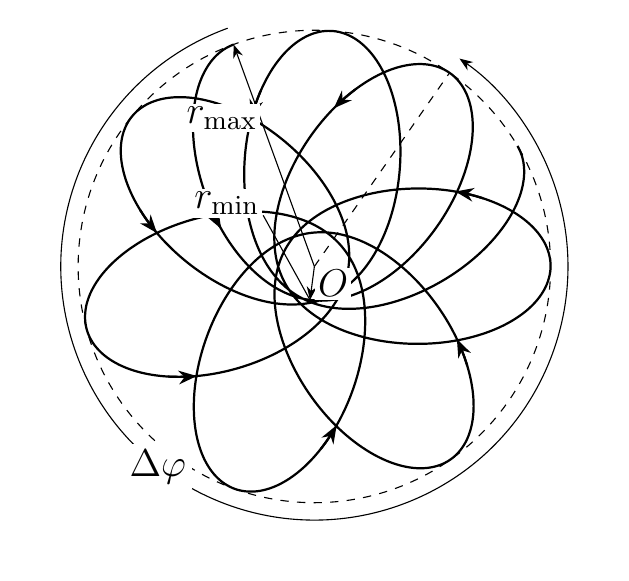
\begin{tikzpicture}[>=Stealth,thick,every node/.style={font=\fontsize{14}{18}\selectfont}]
  % r=p/(1+e cos(k phi)), with e=.75, p=.75, k=1.18.
  % This illustrative rosette has r_min=3/7, r_max=3 and Delta phi=360/k.
  \def\k{1.18}
  \draw[dashed,thin] (0,0) circle (3);
  \draw[
    domain=0:{8*360/\k},samples=1800,smooth,variable=\t]
    plot ({(.75/(1-.75*cos(\k*\t)))*cos(110+\t)},
          {(.75/(1-.75*cos(\k*\t)))*sin(110+\t)});
  \foreach \ang in {45,330,635,940,1245,1550,1855,2160} {
    \draw[->,domain={\ang-3}:{\ang+3},samples=8,variable=\t]
      plot ({(.75/(1-.75*cos(\k*\t)))*cos(110+\t)},
            {(.75/(1-.75*cos(\k*\t)))*sin(110+\t)});
  }
  \draw[thin,->] (0,0) -- (110:3) node[pos=.67,left,fill=white,inner sep=1pt] {$r_{\max}$};
  \draw[thin,->] (0,0) -- ({110+180/\k}:{3/7});
  \node[anchor=east,fill=white,inner sep=1pt] at (-.65,.8) {$r_{\min}$};
  \draw[thin] (-.65,.65) -- ({110+180/\k}:{3/7});
  \node[below right,fill=white,inner sep=1pt] at (0,0) {$O$};
  % Adjacent apocentres are separated by Delta phi=360/k (counterclockwise).
  \draw[thin,dashed] (0,0) -- ({110+360/\k}:3);
  \draw[thin,->] (110:3.22) arc[start angle=110,end angle={110+360/\k},radius=3.22];
  \node[fill=white,inner sep=2pt] at (232:3.23) {$\Delta\varphi$};
\end{tikzpicture}
\end{document}
